% !TEX root = catron-dissertation.tex
\epstopdfsetup{outdir=./images/04_basic_filtering/}

% //TODO:Check Line Numbers of Listings Reference

\chapter{Basic Wavefront Filtering Techniques}
\label{chap:wavefront_filtering}
This chapter will examine some basic wavefront filtering techniques for removal of undesired content from an optical wavefront measurement using a synthetically generated wavefront.
These basic filtering techniques are based on performing a dispersion analysis in order to compute the optical wavefronts spectral content in both time and space.
These techniques are primarily designed for preforming a quick analysis of measured data with some knowledge of the corruption that is present or some user intervention.
It is also likely to remove some desired wavefront components and/or retain some of the measurement corruption.

\section{Dispersion Analysis}
The dispersion analysis as used in this paper is a method for calculating the power spectral density of an optical wavefront in both time and space.
The dispersion plot of a two-dimensional optical wavefront that varies over time is three-dimensional scalar array that lays in temporal (Hz) and spacial ($m^{-1}$) frequency space.
Structures in the dispersion plot lay along a plane that represents its velocity in both $x$ and $y$ directions.
A simple visualization of this is shown in Figure \ref{fig:04_simple_dispersion}.
\begin{figure}
 \centering
 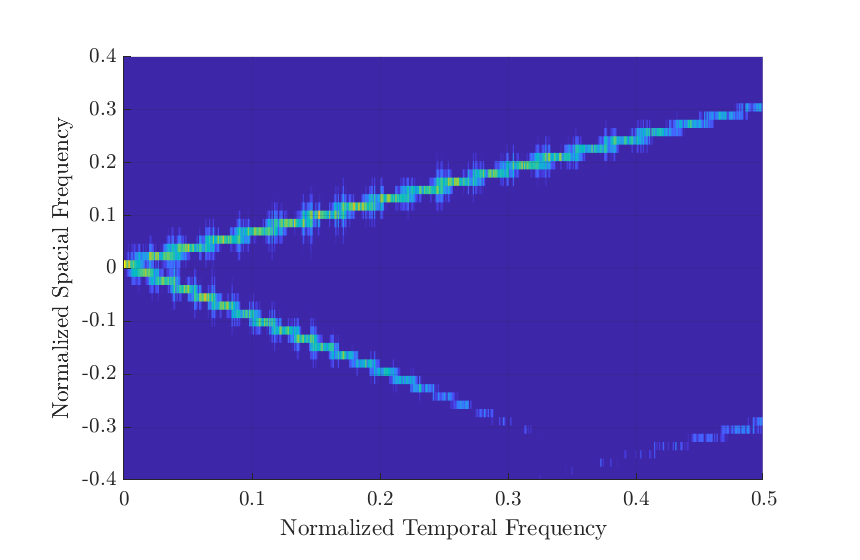
\includegraphics{../matlab/04_basic_filtering/simple_dispersion.eps}
 \caption{A simplified dispersion plot.  Simulation of two broadband plane waves traveling in opposite directions through a one-dimensional wavefront.}
 \label{fig:04_simple_dispersion}
\end{figure}
This simple representation is a simulated one-dimensional wavefront (containing spatial data in only one dimension) that consists of two broadband planar wave structures, one that travels in the negative x-direction while the other in the positive x-direction at 5/3 the speed.
The slope of the structures are inversely related to their velocities when represented with the temporal frequency along the x-axis.
The wave structure traveling in the positive x-direction has much higher frequency content, higher so than the temporal Nyquist frequency and gets aliased into the negative x-direction.
Depending on the filtering methods used, this aliased information can be added on to both ends of the dispersion array in the temporal direction to artificially increase the temporal sample rate of the system.
In this simplified version with the exception of the aliased data and overlap region, these two flow structures can easily be separated into two distinct wavefront components when analyzing the wavefront in frequency space.
\textcolor{red}{I need to add a short discussion on this artificial sample rate increase that can be done at the end of the chapter.}

This dispersion plot can be displayed in a different way, see Figure \ref{fig:04_simple_dispersion_vel}, such that the y-axis represents the velocity of structure if a linear trend between the spatial and temporal frequencies and velocity is assumed.
\begin{figure}
 \centering
 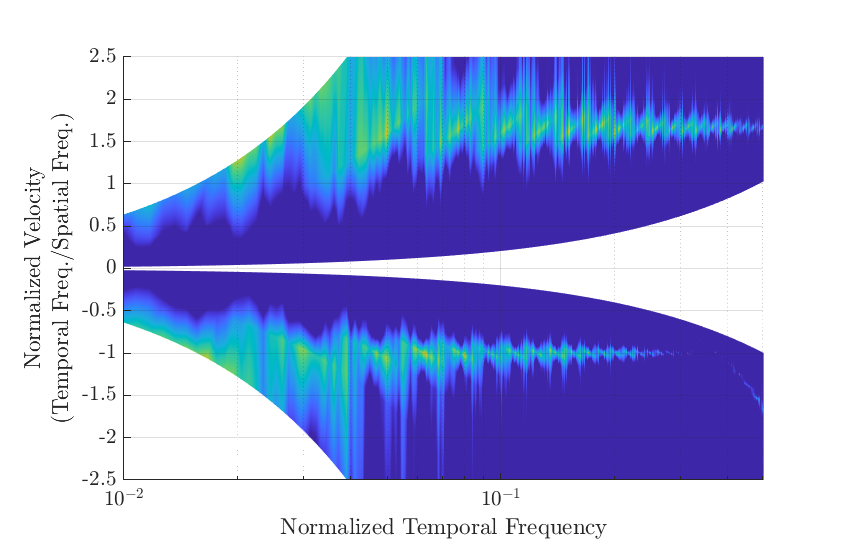
\includegraphics{../matlab/04_basic_filtering/simple_dispersion_vel.eps}
 \caption{Alternative representation of the simplified dispersion plot.  Simulation of two broadband plane waves traveling in opposite directions through a one-dimensional wavefront.}
 \label{fig:04_simple_dispersion_vel}
\end{figure}
Here both waves that are traveling in either direction are clearly discernible, even to low frequencies and allows for the direct reading of the velocity of the group of waves.
One issue with this representation is that the aliased data does not show up as a constant velocity as could be interpreted by the standard dispersion plot given that both lines have the same slope although different y-intercept.

While these plots only show information in the x-spatial/temporal plane, the analysis can be performed in the y-spatial/temporal plane or even three-dimensional representations as shown in Figure \ref{fig:04_dispersion_real}.
\begin{figure}
 \centering
 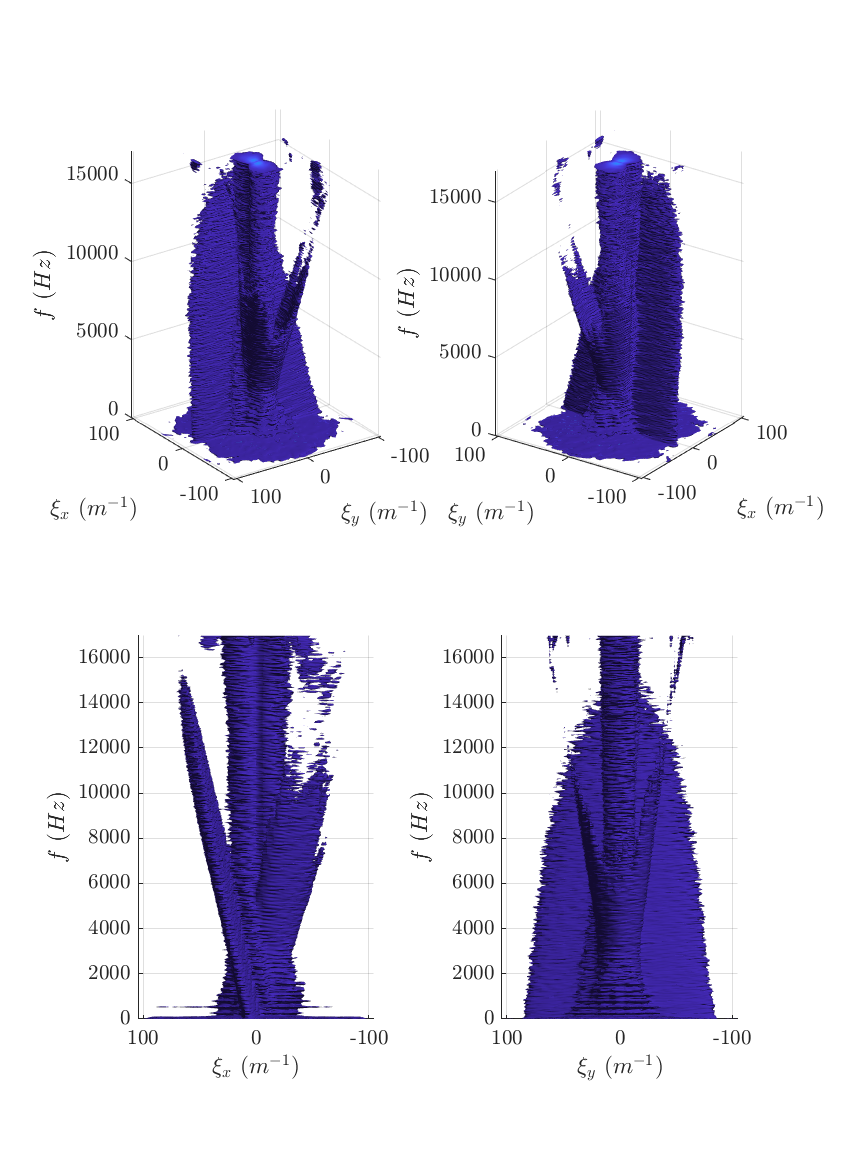
\includegraphics{../matlab/04_basic_filtering/dispersion_real.eps}
 \caption{Dispersion analysis isosurface at a value of $10^{-13}$ $\mu m^2/Hz/m^{-2}$ from two different views.  The isosurface encompasses 99.5\% of the power of the optical disturbances.}
 \label{fig:04_dispersion_real}
\end{figure}
This figure shows an isosurface, which encompasses about 99.5\% of the power, of a measured data set where there are several different prominent structures present.
For additional clarity the various structures are  depicted and colored in Figure \ref{fig:04_synthetic_dispersion_input} for a synthetically generated wavefront that will be discussed later.
The wing shaped structure contains the aero-optical signal of the boundary layer and free-stream turbulence (the red region).
The figure-eight shaped column (the blue region) structure is a collection of spatially stationary modes likely related to measurement noise, while the partial cone is the acoustic duct modes inside the test section (the magenta region).
The large structure near zero-temporal frequency is a combination of vibrations and acoustic contamination, especially around the blade-pass frequency and associated harmonics (the green region).
The last major structure present at zero-temporal frequency and is associated with the mean-lensing of the optical wavefront (the yellow region).

\section{Dispersion Calculation}
As the dispersion analysis is just an extension of the typical power spectra calculation,
\begin{equation}
 S_{xx} = \frac{|\fft(x(t))|^2}{N\cdot f_{samp}} \textrm{,}
 \label{eqn:04_basic_sxx}
\end{equation}
to multiple dimensions, where $\fft$ is the Fast Fourier Transform function, $N$ is the number of points in the transform, $f_{samp}$ is the sample rate, and $S_{xx}$ is the double sided power spectra.
Note, that this form of the equation is for use with MATLAB's way of computing the FFT.
The frequency range goes from $0$ to $f_{samp}\cdot(1-1/N)$ in steps of $f_{samp}/N$ and if the function \lstinline{fftshift} is used on the \lstinline{fft} output the range is shifted to between $-f_{samp}/2$ and $f_{samp}\cdot(1/2-1/N)$ with the same frequency step size.

Because the FFT calculation assumes the signal is periodic, spectral leakage can occur when the signal is not an integer number of wavelengths long.
To minimize this spectral leakage, windowing functions are employed which typically force the end points of the signal to zero.
The Hann window,
\begin{equation}
 w(t) = 1/2\left[1-\cos\left(\frac{2\pi t}{T}\right)\right] \textrm{,}
 \label{eqn:04_hann_window}
\end{equation}
is one of the more commonly used windowing functions where $w(t)$ is the window function, $t$ is the time at a given sample, and $T$ is the total sample time.
Since the windowing of a data set changes the signal energy some correction is needed to be applied.
For an arbitrary windowing function the correction factor, $c_w$, is
\begin{equation}
 c_w = \frac{1}{\sqrt{\sum w^2(t)/N}} \textrm{.}
 \label{eqn:04_window_correction}
\end{equation}
For a Hann window this correction factor approaches $\sqrt{8/3}$ as $N$ goes to infinity.
When the equaiton \ref{eqn:04_basic_sxx} is combined with a windowing function and associated correction the double sided power spectra equation in one dimension becomes
\begin{equation}
 S_{xx} = c_w\cdot\frac{|\fft\{x(t)\cdot w(t)\}|^2}{N\cdot f_{samp}} \textrm{.}
 \label{eqn:04_windowed_sxx}
\end{equation}
A simple MATLAB function for computing the power spectra of a one-dimension signal with an arbitrary windowing function is shown in Listing \ref{code:sc_simpleSXX}.

For measurements with multiple spatial and temporal dimensions the Fast Fourier Transform is just applied $n$-times where $n$ is the total number of dimensions, with each application in a different dimension,
\begin{equation}
 \fftn(x) = \fft(\fft(\cdots\fft(\fft(x,1),2)\cdots,n-1),n) \textrm{,}
 \label{eqn:04_fftn}
\end{equation}
where $\fft(x,n)$ is the Fast Fourier Transform of $x$ in the $n^{th}$ dimension.
For a $n$-dimensional array the power spectra the function becomes,
\begin{equation}
 \mathbf{S_{xx}} = c_w\cdot\frac{|\fftn\{f(\mathbf{x})\cdot w(\mathbf{x})\}|^2}{\prod{\overrightarrow{N}\cdot \overrightarrow{f}_{samp}}} \textrm{,}
 \label{eqn:04_sxxn}
\end{equation}
where $\mathbf{S_{xx}}$ is the $n$-dimensional power spectra array or dispersion array, $f(\mathbf{x})$ is a $n$-dimensional set of data, $w(\mathbf{x})$ is a $n$-dimensional windowing function, $\overrightarrow{N}$ is a vector denoting the number of elements in each dimension, $\overrightarrow{f}_{samp}$ is a vector denoting the sample rate in each dimension, and
\begin{equation}
 c_w = \frac{1}{\sqrt{\sum w^2(\mathbf{x})/\prod{\overrightarrow{N}}}} \textrm{.}
 \label{eqn:04_windown}
\end{equation}
A simple MATLAB code for calculating the dispersion of $x$ with an arbitrary windowing function is shown in Listing \ref{code:sc_simpleSXXn}.

The optical wavefronts used throughout this paper are round apertures with no additional obscurations and is constant throughout the sample period.
This allows the windowing function to be split into two separate components,
\begin{equation}
 w(\mathbf{x}) = w_t(t)\cdot w_s(x,y) \textrm{,}
 \label{eqn:04_window_sep}
\end{equation}
the temporal windowing function, $w_t(t)$, and the spatial windowing function, $w_s(x,y)$.
Both the temporal and spatial windowing functions used in this paper are Hann windows.
The temporal window used the function shown in Equation \ref{eqn:04_hann_window}, while the spatial windows use on of two modified windows which have a value of one furthest from the edge of an aperture or zero at the edge of an aperture.
The first of these spatial windows is for a circular aperture an is based normalized radius, $\rho_N$, of the aperture,
\begin{equation}
 w_s(\rho_N) =
 \begin{cases}
  \frac{1+\cos(\pi\cdot\rho_N)}{2} & \textrm{if } \rho_N < 1 \\
  0                                & \textrm{otherwise.}
 \end{cases}
 \label{eqn:04_window_space}
\end{equation}

For second spatial windowing function is for an arbitrary shaped aperture and is computed by finding the minimum distance from any point within the aperture to a point on the edge of the aperture,
\begin{equation}
 d_{min}(x,y) = \min\left\{\sqrt{(x-x_{O})^2+(y-y_{O})^2}\right\} \textrm{,}
 \label{eqn:04_window_space_arb_dist}
\end{equation}
where $O$ denotes the set of points outside of the aperture.
This distance is then normalized by the maximum value resulting in,
\begin{equation}
 w_s(x,y) = \frac{1+\cos\left\{\pi\cdot\left(1-d_{min}^{norm}(x,y)\right)\right\}}{2} \textrm{.}
 \label{eqn:04_window_space_arb}
\end{equation}

\section{Synthetic Wavefront Generation}
In order to best understand how some basic filters preform on a set of data, a fully known synthetic wavefront was generated such that all of the various components could be generated separately with the combined product filtered and compared to the synthetic wavefront containing only relevant aero-optical data.
This is done by creating an input dispersion plot where each source component is separately generated with parameters that can be modified to alter the output signal as necessary.
Signals that are assumed to be statistically independent are converted into dimensional space separately and then summed together.
While signals that are assumed to be related to one another (such as the sound and vibration components) are summed together in frequency space.
Figure \ref{fig:04_synthetic_dispersion_input} shows the input dispersion plot with each signal component separately colored.
\begin{figure}
 \centering
 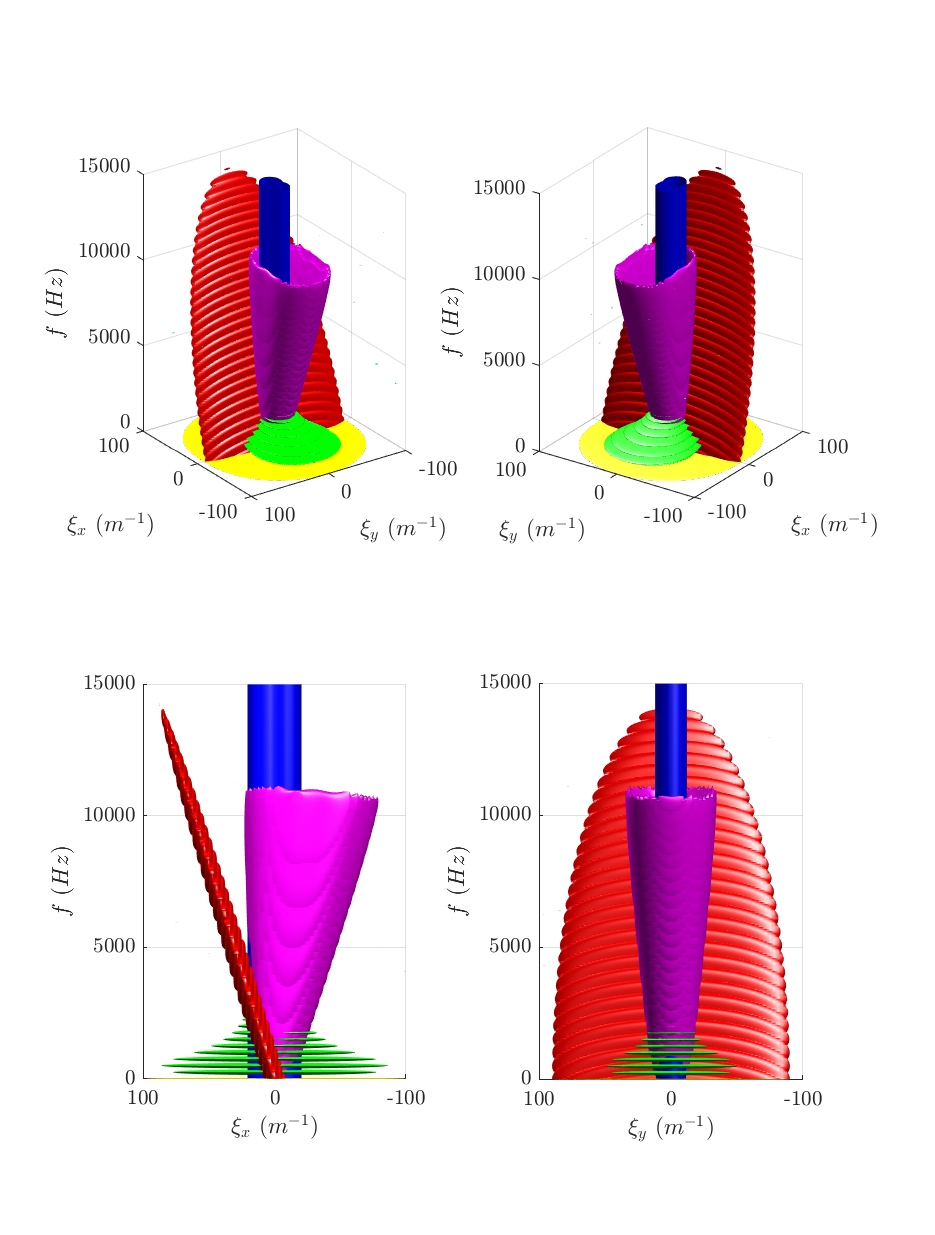
\includegraphics{../matlab/04_basic_filtering/synthetic_wavefront.eps}
 \caption{Synthetic wavefront input dispersion plot of an aero-optical signal and various signal corruption components.  The aero-optical signal is shown in red, the stationary modes in blue, duct acoustics in magenta, blade-passing frequency related corruption in green, slowly varying mean-lensing in yellow, and background in cyan.}
 \label{fig:04_synthetic_dispersion_input}
\end{figure}
The aero-optical signal is shown in red, the stationary modes in blue, duct acoustics in magenta, blade-passing frequency related corruption in green, slowly varying mean-lensing in yellow, and background in cyan.

Wavefronts were generated to approximate the sample conditions in that the data presented in Figure \ref{fig:04_dispersion_real} were measured with.
The sample rate was 200 m$^{-1}$ with 64 ($2^6$) samples in the spatial dimensions and 30,000 Hz with 8192 ($2^{13}$) samples in the temporal dimension.
The speed of sound was chosen to be 340 m/s, with a Mach number of 0.6, and a boundary layer velocity of 163.2 m/s ($0.8U_\infty$).

The general process of developing most of the component signals was to determine an approximate shape, normalize it in the appropriate dimensions, and scale the result by using a function derived from a hyperbola,
\begin{equation}
 \frac{\log_{10}(WF)-b}{b^2}-\frac{\xi_{\rho_N}^2}{a^2} = 1 \textrm{,}
 \label{eqn:04_scaling_hyperbola}
\end{equation}
such that the signal strength at unity of the normalized radial frequency, $\log_{10}(WF(\xi_{\rho_N}=1))$, and the limiting slope, $a/b$, are inputs.
This results in the signal strength of the wavefront being
\begin{equation}
 \log_{10}(WF) = b-\sqrt{\frac{\xi_{\rho_N}^2}{m^2}+b^2} \textrm{,}
 \label{eqn:04_wavefront_strength}
\end{equation}
where
\begin{equation}
 b = \frac{1}{2\log_{10}(WF(\xi_{\rho_N}=1))}\cdot\left(\log_{10}(WF(\xi_{\rho_N}=1))^2-\frac{1}{m^2}\right) \textrm{.}
 \label{eqn:04_wavefront_strength_b}
\end{equation}
The code used to generate the synthetic wavefront used in this section is shown in Listing \ref{code:sc_synthetic_wavefront}.

\subsection{Aero-Optical Signal}
The aero-optical signal which is approximating an optical beam passing through a boundary layers normal to each of the test section walls.
This signal was approximated by creating an ellipsoid in the plane of the feature's velocity and normalizing the radius by some arbitrary factors to roughly match the shape of the measured dispersion plot shown in Figure \ref{fig:04_dispersion_real}.
The dispersion magnitude was then calculated by applying Equation \ref{eqn:04_wavefront_strength}, with relevant code shown on Lines 19-30 of Listing \ref{code:sc_synthetic_wavefront}.
In Figure \ref{fig:04_synthetic_dispersion_input} the aero-optical signal is shown in red.

\subsection{Stationary Mode Signals}
The stationary modes in Figure \ref{fig:04_dispersion_real} appear to be temporally white-noise with the spatial frequencies forming an epicycloid of $k=2$.
This shape was further simplified using a single trigonometric function to represent the normalization function of the radial spatial frequency,
\begin{equation}
 \xi_{\rho_N} = \frac{\xi_\rho}{\xi_{\rho_0}\sqrt{10-6\cos{(2\xi_\theta)}}} \textrm{,}
\end{equation}
this makes an epicycloidal like shape which has a smooth derivative.
This dispersion component is shown in blue in Figure \ref{fig:04_synthetic_dispersion_input} and the relevant code shown in Lines 61-66 of Listing \ref{code:sc_synthetic_wavefront}.

\subsection{Sound \& Vibration Signals}
The sound \& vibrating component signals are comprised of two parts.
The first of these is the blade-passing frequency and its harmonic disturbances (shown in green in Figure \ref{fig:04_synthetic_dispersion_input}) and the second is the acoustic duct modes (shown in magenta).
Like the stationary modes, the blade-passing frequency disturbances were modeled with the simplified epicycloid narrow-band disc and each harmonic was modulated by using a low-pass filter offset to the blade-passing frequency.
The code for the blade-passing frequency disturbances is shown in Lines 97-113 of Listing \ref{code:sc_synthetic_wavefront}.

The acoustic duct mode disturbances form a cone which in the $f-\xi_x$ plane is defined by the lines $u\pm c$, while in the $f-\xi_y$ plane is defined by the speed of sound.
At each temporal frequency step an ellipse was defined based on the constraining lines and the distance to that ellipse used to calculate a normalized radial frequency.
The strength of the disturbance was decreased logarithmically in temporal frequency as shown in the code in Lines 183-200 of Listing \ref{code:sc_synthetic_wavefront}.

\subsection{Mean Lensing Signal}
The mean-lensing signal (shown in yellow in Figure \ref{fig:04_synthetic_dispersion_input}) uses a stretched version of the simplified epicycloid and represents the slowly varying spatial disturbance.
The relevant code is shown on Lines 144-152 of Listing \ref{code:sc_synthetic_wavefront}.

\subsection{Background Noise Signal}
The background noise disturbance (with a few small spots shown in cyan in Figure \ref{fig:04_synthetic_dispersion_input}) was the only component that did not use the hyperbola to scale the signal but instead was just normally distributed random noise with a mean noise level and deviation as inputs.
The relevant code is shown in Lines 230-234 of Listing \ref{code:sc_synthetic_wavefront}.

\subsection{Synthetic Wavefront Creation}
A synthetic signal can be created from a power spectra by solving for $x$ in Equation \ref{eqn:04_basic_sxx} and using the Inverse Fast Fourier Transform,
\begin{equation}
 x(t) = \real\left[\ifft\left\{\sqrt{S_{xx}\cdot N\cdot f_{samp}}\cdot\exp{i\phi}\right\}\right] \textrm{,}
 \label{eqn:04_ifft}
\end{equation}
where $\real$ is the real component and $\phi$ is a random set of phases for each point in the measurement space.
As shown previously this relation can be extended into $n$-dimensions,
\begin{equation}
 f(\mathbf{x}) = \real\left[\ifftn\left\{\sqrt{\mathbf{S_{xx}}\cdot\prod{\overrightarrow{N}\cdot \overrightarrow{f}_{samp}}}\cdot\exp{i\mathbf{\phi}}\right\}\right] \textrm{.}
 \label{eqn:04_ifftn}
\end{equation}
Care should be taken when constructing the random set of phases, as the zero-frequency component has zero phase and the phases on either side of it are conjugates of one another.
The code for creating a wavefront from a dispersion plot is shown in Lines 336-340 of Listing \ref{code:sc_synthetic_wavefront} and is specifically creating the wavefront for the aero-optical signal but other signals are generated using the same basic code.
Note that the first three lines are to get the set of phases properly configured that creates conjugate phases rotated about the origin.

It was assumed that the aero-optical signal, the stationary modes, and the background noise were statistically independent of one another and the sound and vibration combination of modes and as such could be separately transformed into physical space.
While the components of the sound and vibration sources, the blade-passing frequency, the acoustic cone, and the mean-lensing, were assumed to be related to one another and thus were summed together in frequency space prior to being transformed into physical space.
Once the separate components were in physical space the total wavefront was obtained by summing up the separate components with the aero-optical signal being a separately saved along side the total wavefront.
Some frames from the synthetic wavefront are shown in Figure \ref{fig:04_synthetic_frames} with the total wavefront shown on top and the aero-optical only signal shown on the bottom.
\begin{figure}
 \centering
 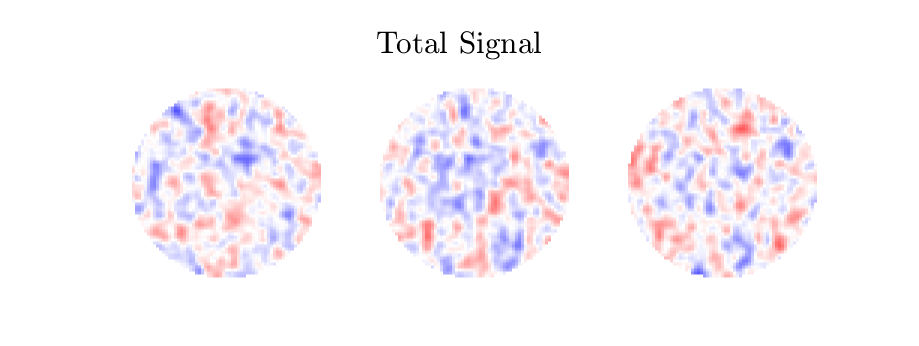
\includegraphics{../matlab/04_basic_filtering/synthetic_frames_total.eps}
 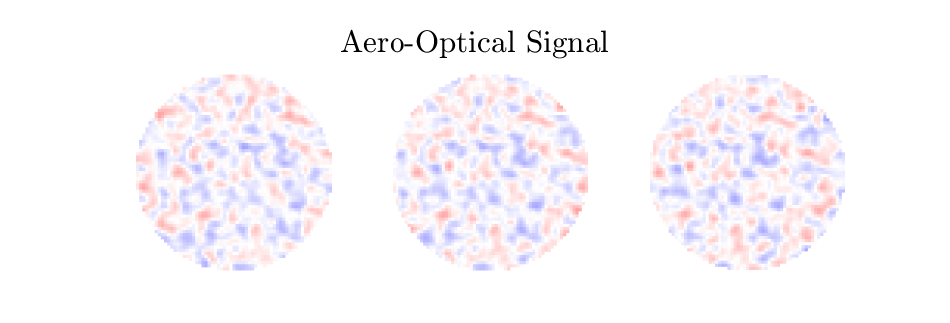
\includegraphics{../matlab/04_basic_filtering/synthetic_frames_ao.eps}
 \caption{Sample frames from the synthetic wavefront with the total wavefront signal on top and the aero-optical only signal bottom.  Flow is from right to left.}
 \label{fig:04_synthetic_frames}
\end{figure}
Flow is from right to left.
The aero-optical signal is often times noticeable in the total wavefront signal, but can be easily overpowered by the various contamination sources.

\subsection{Comparison to Measured Data}
A dispersion plot of the total synthetic wavefront is shown in Figure \ref{fig:04_dispersion_synthetic}.
\begin{figure}
 \centering
 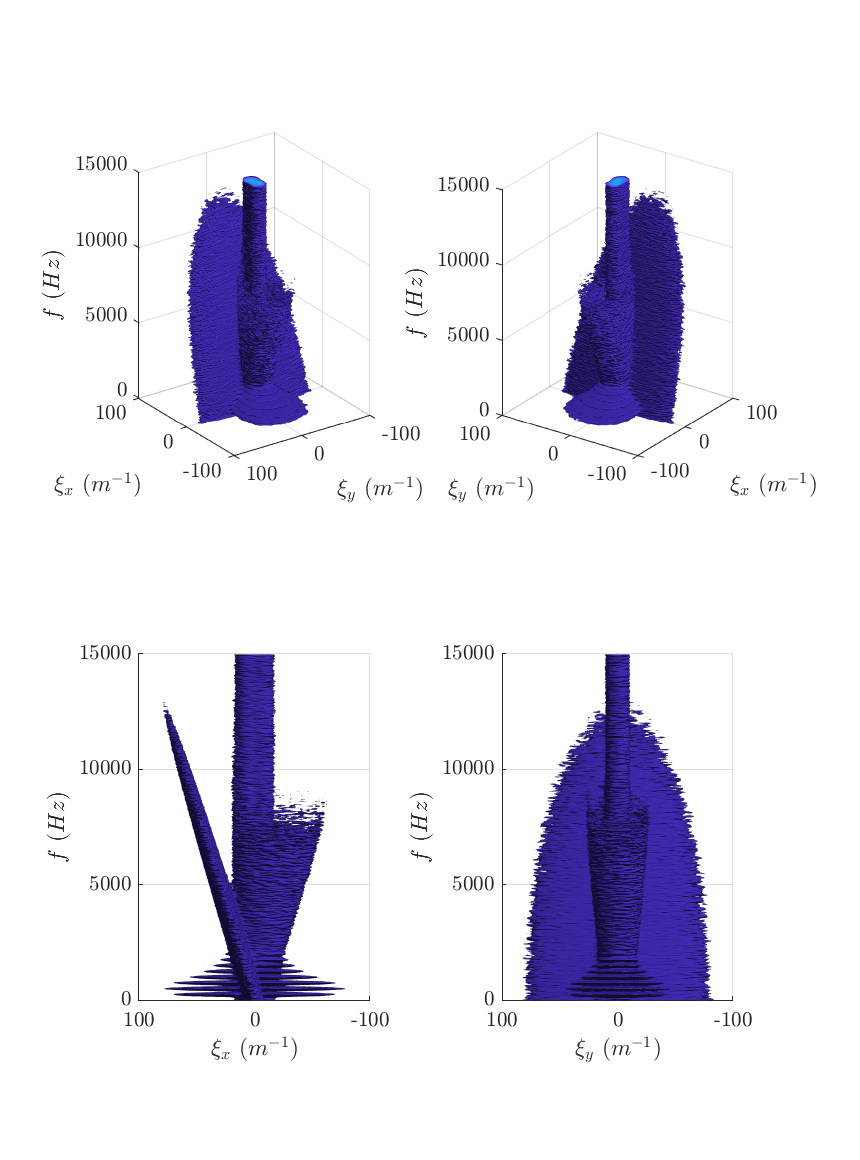
\includegraphics{../matlab/04_basic_filtering/dispersion_synthetic.eps}
 \caption{Synthetic wavefront output dispersion plot of an aero-optical signal and various signal corruption components.}
 \label{fig:04_dispersion_synthetic}
\end{figure}
In this view the aero-optical signal is more noticeable but there still remains some significant overlap with the various contamination sources.
While the mean-lensing component is not as visible in this isosurface, the rest of the dispersion plot in a good representation of the input dispersion plot shown in Figure \ref{fig:04_synthetic_dispersion_input}.
The blade-passing frequency was depicted as symmetric in the synthetic wavefront while measured data (shown in Figure \ref{fig:04_dispersion_real}) shows more signal on the side traveling in the direction of flow.
The harmonics of the BPF are more on the upstream traveling side of the dispersion and are a little less pronounced in the measured data.
The total synthetic wavefront has a spatial time-averaged RMS of $0.0112\pm0.0006\mu m$ with the aero-optical only signal having a spatial time-averaged RMS of $0.0073\pm0.0003\mu m$.
The measured wavefront presented in Figure \ref{fig:04_dispersion_real} had a spatial time-averaged RMS of $0.0874\pm0.0263\mu m$.
The overall spatial RMS of the synthetic wavefront was $12.8\%$ when compared to the measured wavefront indicating that the algorithms used to generate the wavefront are not representative of reality and can provide a future path of research in order to produce more realistic synthetic wavefronts.
\textcolor{red}{Double Check line numbers for the Listings.}


\section{Filtering Basics}
A filter is a function, $G(\mathbf{\omega})$, that describes the gain a signal will experience in frequency space.
In the simplest case, the filtered signal is the inverse Fourier transform of the gain multiplied by the Fourier transform of the signal.
Additionally, a windowing function, $W(\mathbf{x})$, can be used to help suppress finite sampling effects,
\begin{equation}
 f_F(\mathbf{x}) = \real\left(\frac{\ifftn[G(\mathbf{\omega})\cdot\fftn\{f(\mathbf{x})\cdot W(\mathbf{x})\}]}{W(\mathbf{x})}\right) \textrm{,}
 \label{eqn:04_filter_function}
\end{equation}
where $f$ is the signal function and $f_F$ is the filtered signal.
Depending on the windowing function some data could be destroyed during this process if there is a zero present due to the possibility of dividing by zero.

A basic MATLAB code for applying a filter to a wavefront using a separate function for both generating and applying the gain function which is presented in Listing \ref{code:sc_basic_wavefront_filters}.
This code generates a windowing function as described by Equations \ref{eqn:04_hann_window}, \ref{eqn:04_window_sep}, and \ref{eqn:04_window_space_arb}.
The temporal windowing function was generated with an additional two terms such that the end points which are equal to zero could be removed to prevent the first and last frames from being destroyed.
Likewise, the spatial window used the arbitrary aperture function which ensures that all of the points inside of the aperture are non-zero.
In some cases, a windowing function was not used due to filtered wavefront having a far greater magnitude in some places despite the precautions used.
The filter presented in this code sample is a second order temporal high-pass filter with a cut-off frequency of 2000 Hz.
The function \lstinline{WFfilter} takes input based on a normalized cut-point in reference to the sample rate.

\section{Temporal Filter Methods}
The methods presented in this section are based on Butterworth filters \cite{Butterworth-1930-DvDrjKha} but could easily be extended to other types of filters.
The basic gain function,
\begin{equation}
 G(f) = \frac{1}{\sqrt{1+\left(\frac{f}{f_c}\right)^{\pm2n}}} \textrm{,}
 \label{eqn:04_butterworth}
\end{equation}
where $f_c$ is the cut-off frequency, $n$ is the filter order (number of filters in a series), and $\pm$ represents either a low-pass ($+$) or high-pass ($-$) filter.
In this particular formulation, only the magnitude is attenuated, circuit based Butterworth filters or their digital copies will have some variable phase attenuation as well.
Additionally, a band-pass filter can be constructed by placing a low-pass in series with a high-pass filter and a band-stop by placing the two types in parallel.

As a large portion of the wavefront contamination is at low frequencies, a high-pass filter is the most useful in temporal space for removing unwanted contamination, as shown in Figure \ref{fig:04_filter_temporal}.
\begin{figure}
 \centering
 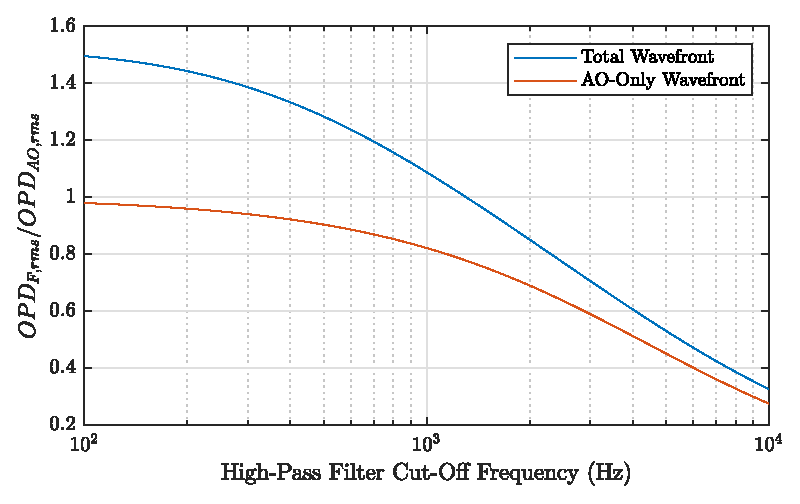
\includegraphics{../matlab/04_basic_filtering/filter_temporal.eps}
 \caption{OPD time-averaged spatial-RMS of high-pass temporal filters relative to the aero-optical only unfiltered wavefront.}
 \label{fig:04_filter_temporal}
\end{figure}
This figure shows the time-averaged spatial-RMS of both the total and aero-optical only wavefronts with various cut-off high-pass filters relative to that of the aero-optical only wavefront unfiltered.
The total wavefront ratio crosses unity around 1200 Hz, which is about halfway between the second and third harmonic of the blade-passing frequency in this simulated wavefront.
While approximately 75\% of the aero-optical signal remains at this cut-off frequency, that difference is made up by the remaining contamination.
This can provide a computationally cheap way estimating the aero-optical portion of the wavefront for calculations that rely on the spatial-RMS of a wavefront.
While it is easy to determine a cut-off frequency for this synthetic wavefront, a measured wavefront will likely take some knowledge or expectation of the contamination that is present in the measurement.

An example of band-pass and band-stop filtering is shown if Figure \ref{fig:04_filter_temporal_bandpass}.
\begin{figure}
 \centering
 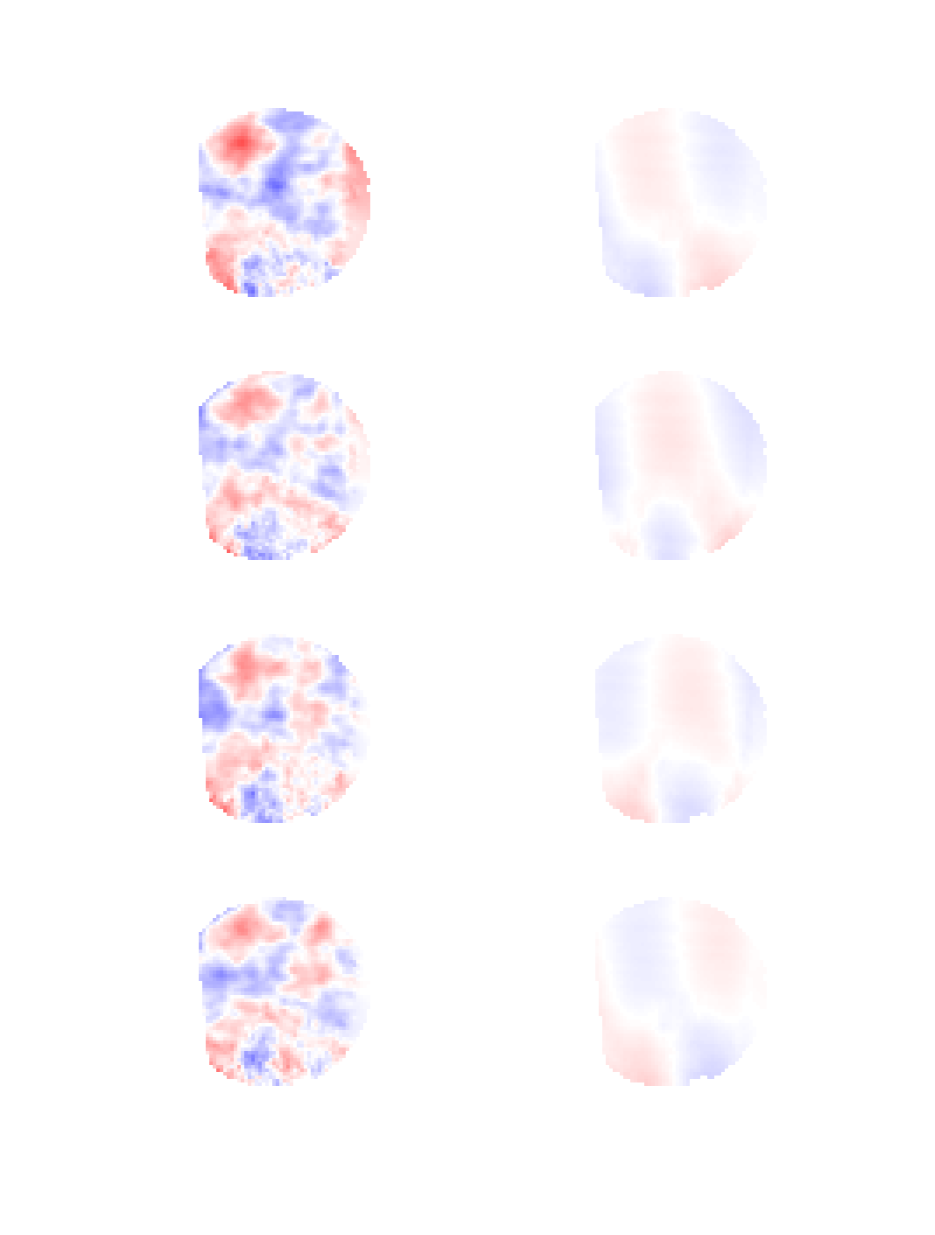
\includegraphics{../matlab/04_basic_filtering/filter_temporal_bandpass.eps}
 \caption{Measured wavefronts filtered at the blade-passing frequency (532$\pm$10 Hz).  The left column is band-stop filtered while the right is band-pass filtered.}
 \label{fig:04_filter_temporal_bandpass}
\end{figure}
The figure shows measured data that is band-stop filtered in the left column and band-pass filtered in the right column in several different frames.
The flow is from right-to-left and the band-pass filtered wavefront clearly shows upstream-moving optical disturbances associated with acoustic duct modes traveling upstream from the fan.
The band-stop shows a much slower moving optical disturbance that is in general moving in the direction of the flow, but it still possess the optical disturbances of the blade-pass frequency harmonics.

One thing of note, MATLAB's builtin filter functions only work in one-dimension of frequency space and are unable to determine the direction that a signal is traveling.
They also only apply the filter to the positive frequencies and zero-out the negative ones which both reduces the signal by two and also switches all disturbances to moving in the same direction.
So even for a filter that operates in one-dimension, it is best to apply the filter over both positive and negative frequencies to the n-dimensional Fourier transform in order to preserve the direction of travel of a signal.
This additionally allows several filters to be applied in series with one another without having to perform a Fourier and inverse Fourier transform for each successive filter.
\textcolor{red}{I should maybe show this matlab filter issue in an appendix.}

Some additional uses of temporal filters would be in sizing and/or designing an adaptive optics system.
A low-pass filter with a cut-off at the bandwidth of either a fast-steering or deformable mirror would help determine the signal that a system would need to reject.
A control system may need to have the bandwidth reduced in order to keep a mirror's travel within limits.
While a high-pass filter would inform designers of the remaining optical aberrations that cannot be corrected.




\section{Upstream/Downstream Moving}
For the filtering of upstream and downstream moving optical disturbances a logistic function was chosen,
\begin{equation}
 f(x) = \frac{1}{1+\exp\{-kx\}} \textrm{.}
 \label{eqn:04_logistic}
\end{equation}
This function needs to be expanded into two-dimensions ($x$ and $t$) with the filter ideally returning a value of one in both the first and third quadrants and zero otherwise for a filter outputs disturbances moving in the direction of flow.
To accomplish this the logistic curve in each dimension is scaled and offset to output values between negative one and positive one,
\begin{equation}
 G_t(f) = \frac{2}{1+\exp\{-k_tf\}}-1
 \label{eqn:04_logistic_time}
\end{equation}
and
\begin{equation}
 G_x(\xi_x) = \frac{2}{1+\exp\{\pm k_x\xi_x\}}-1 \textrm{,}
 \label{eqn:04_logistic_space}
\end{equation}
where $\pm$ determines whether the filter is obtaining upstream traveling disturbances ($+$) or downstream traveling ($-$).
These two gain functions are then multiplied together and scaled to output values between zero and one,
\begin{equation}
 G(\xi_x,f) = \frac{(G_t\cdot G_x)+1}{2} \textrm{.}
 \label{eqn:04_up_down_filter}
\end{equation}
As the values of $k_x$ and $k_t$ go to infinity an ideal case is obtained.
Downstream traveling disturbances have a gain of one in the first and third quadrants, zero in the second and forth quadrants, and a value of $1/2$ when either frequency is zero.

The dispersion analysis using an ideal downstream moving filter on the synthetic wavefront is shown in Figure \ref{fig:04_filter_downstream} along side the dispersion of the unfiltered wavefront.
\begin{figure}
 \centering
 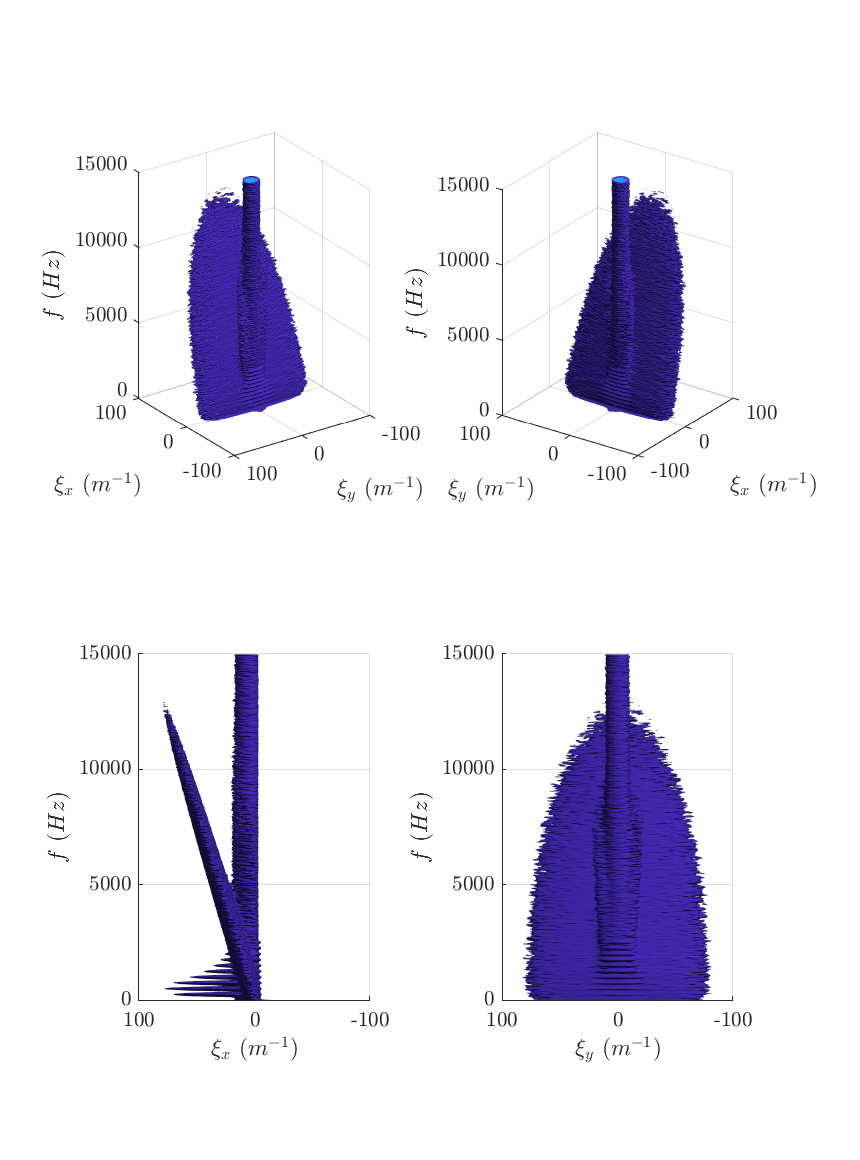
\includegraphics{../matlab/04_basic_filtering/filter_downstream.eps}
 \caption{Dispersion isosurface of the synthetic wavefront with a downstream filter in place.}
 \label{fig:04_filter_downstream}
\end{figure}
All of the upstream traveling disturbances are removed and the disturbances at $\xi_x=0$ m$^{-1}$ are significantly reduced.
Some of the stationary modes remain while only the acoustic and vibration signals that are propagating in the direction of flow remain.
The aero-optical signal is clipped slightly at $\xi_x=0$ due to the spatial width of the signal.
The ratio of the time-averaged spatial-RMS of the filtered signal when compared to the aero-optic only signal was 1.24 while the unfiltered ratio was 1.53.
When the filter was applied to only the aero-optic signal the ratio was 0.96.
This filter method will retain any disturbance that is traveling in the direction of flow.
Even with an ideal filter there is some slight attenuation of the aero-optical signal due to signal having some spectral width that crosses into upstream-moving portion of the dispersion plot.


\section{Velocity Filtering}
The dispersion plot shows flow structures that are traveling at a given speed as having a constant slope.
A plane in the dispersion plot can be used to measure a flow structure's velocity in both $x$ and $y$-directions.
The distance from any given point in the dispersion plot to a plane described by the velocities $v_x$ and $v_y$ can be computed by
\begin{equation}
 d = \frac{|v_x\xi_x+v_y\xi_y-f|}{\sqrt{v_x^2+v_y^2+1}} \textrm{.}
 \label{eqn:04_dist_point_2_plane}
\end{equation}
A low-pass or high-pass filter can then be used to retain only disturbances that are traveling at that velocity, or to exclude those disturbances respectively.

A low-pass velocity-filter of the synthetic wavefront is shown in Figure \ref{fig:04_filter_velocity}.
\begin{figure}
 \centering
 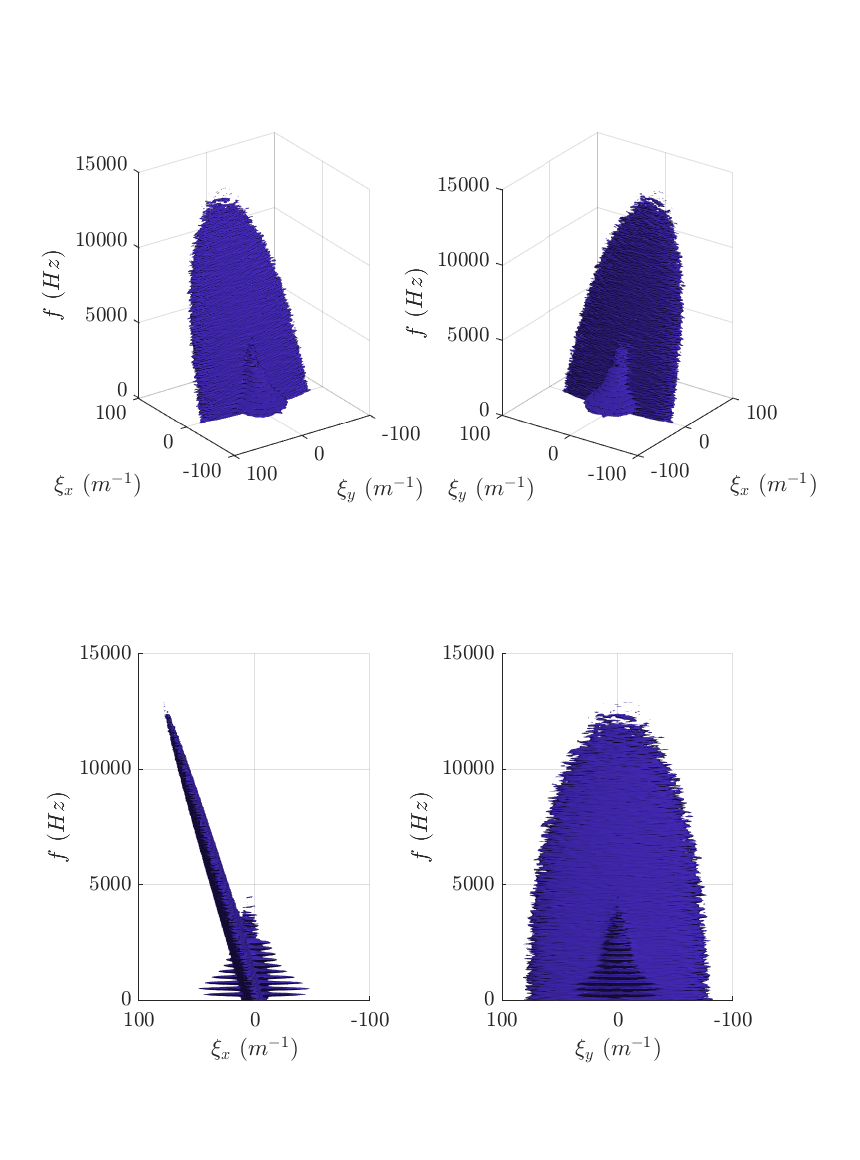
\includegraphics{../matlab/04_basic_filtering/filter_velocity.eps}
 \caption{Dispersion isosurface of the synthetic wavefront with a low-pass velocity-filter in place.}
 \label{fig:04_filter_velocity}
\end{figure}
The filtered dispersion plot shows primarily only the aero-optic signal remains with some additional low-frequency content from the blade-passing frequency and harmonic disturbances as well as some stationary and acoustic disturbances.
The ratio of the time-averaged spatial-RMS relative to that of the aero-optical only signal went from 1.53 in the unfiltered case to 1.01 in the filtered case.
This method can provide a very effective way in quickly estimating the clean spatial-RMS of a contaminated wavefront.

Another use of the synthetic wavefront is measuring the speed of a broadband disturbance such as the aero-optical signal of a boundary layer.
This is done by finding the velocity that maximizes the output spatial-RMS of the velocity filter, see Figure \ref{fig:04_filter_velocity_measure}.
\begin{figure}
 \centering
 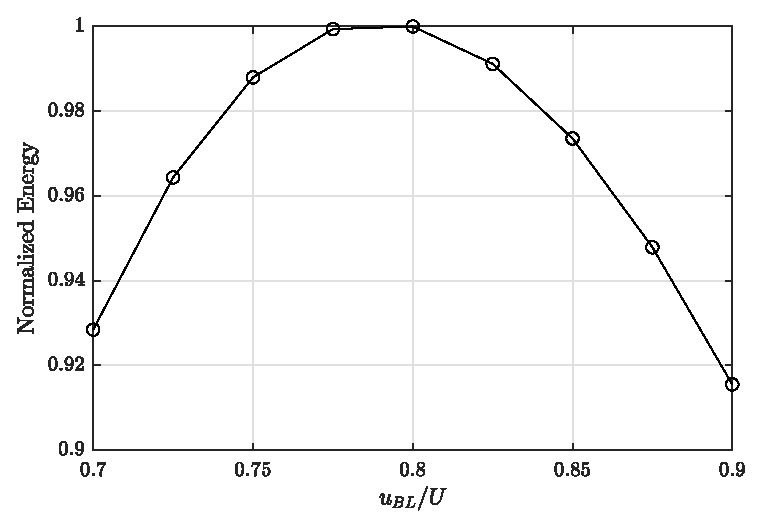
\includegraphics{../matlab/04_basic_filtering/filter_velocity_measure.eps}
 \caption{Velocity low-pass filter used to determine the mean disturbance velocity.  The maximum value corresponds with the actual value used in the creation of the synthetic wavefront.}
 \label{fig:04_filter_velocity_measure}
\end{figure}
In this case boundary layer speed was determined to be 163 m/s which corresponds to the design velocity of the synthetic signal of $0.8U$.
If the velocity range used is to large, a false result can be obtained due to the inclusion of disturbance structures not related to the aero-optical signal.
For signals that have a mean-velocity component that is not aligned with an axis both velocity components can be varied as shown in Figure \ref{fig:04_filter_velocity_real}.
\begin{figure}
 \centering
 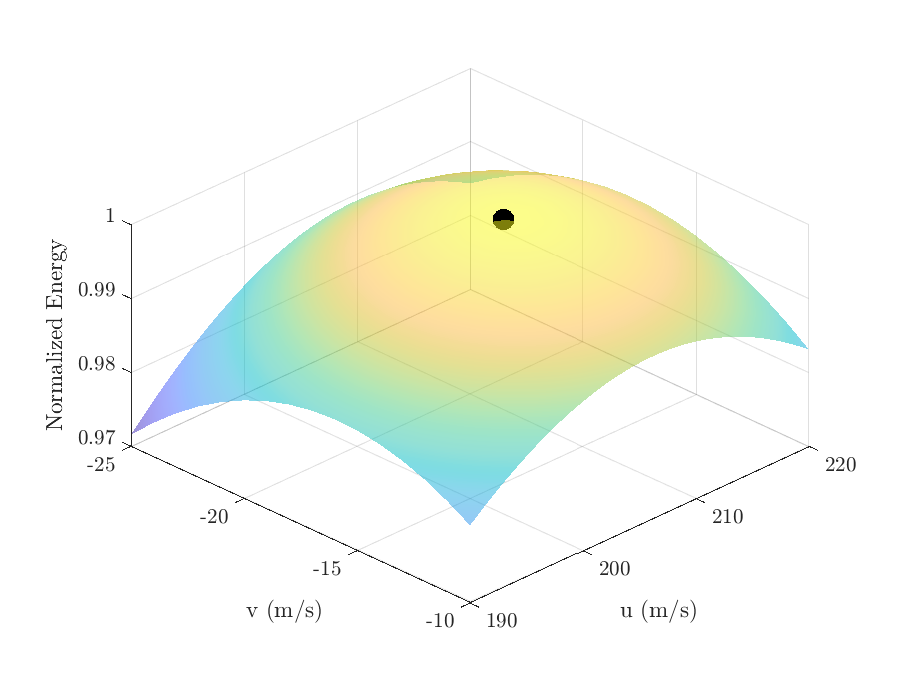
\includegraphics{../matlab/04_basic_filtering/filter_velocity_real.eps}
 \caption{Velocity low-pass filter used to determine the mean disturbance velocity of measured data presented in Figure \ref{fig:04_dispersion_real}.  The velocity in the x-direction was measured to be 207 m/s and -17 m/s in the y-direction.}
 \label{fig:04_filter_velocity_real}
\end{figure}
In this case a variable low-pass velocity filter was employed with a high-pass spatial filter operating in the radial direction.
This helped eliminate some of the low-frequency stationary disturbances as well as some of the disturbances related to the blade-passing frequency.
The velocity was measured using the optical disturbances in the dispersion plot to be approximately 207 m/s in the x-direction and -17 m/s in the y-direction.

\section{Basic Filter Summary}
Three different basic wavefront filters were shown and discussed in this chapter.
The temporal filter is most useful when separating an optical wavefront into frequency bands.
Adaptive optics system performance can be evaluated by using both high-pass and low-pass temporal filters.
High-pass filters can be used to determine a systems performance that cannot be corrected while low-pass filters can be used to sizing the travel of active optical components.
Band-pass filters are helpful in analyzing a wavefront over a narrow-band to examine the optical aberrations at specific frequencies that significantly contribute to the overall optical disturbance.

Filters that separate upstream and downstream-moving disturbances are useful as most of the optical contamination comes from acoustic signals that are traveling upstream form a wind-tunnel fan.
These filters would also be useful for separating out an aero-optical signal that has a broad range of velocities that can occur in a span wise measurement of a boundary layer.
\textcolor{red}{Use some of sontag's data and site his dissertation.}

The velocity filter is the most useful for isolating the aero-optical portion of a wavefront measurement given the aero-optical signal has a fairly narrow and constant velocity range.
By using this filter to maximize the power over a range of velocities it can be used to measure the speed in both x and y-directions of an optical disturbance.
